\documentclass{vgtc}

% set font encoding for PDFLaTeX or XeLaTeX
\usepackage{ifxetex}
\ifxetex
	\usepackage{fontspec}
\else
	\usepackage[T1]{fontenc}
	\usepackage[utf8]{inputenc}
	\usepackage{lmodern}
\fi
\usepackage{graphicx}
\usepackage{float}
\usepackage{cite}

% used in maketitle
\title{Study of freight accross Europe.}
\author{Barbier Jeremy, Bazin Adelme, Paffoni Nina}


\begin{document}
\maketitle

\begin{figure}[H]
\center
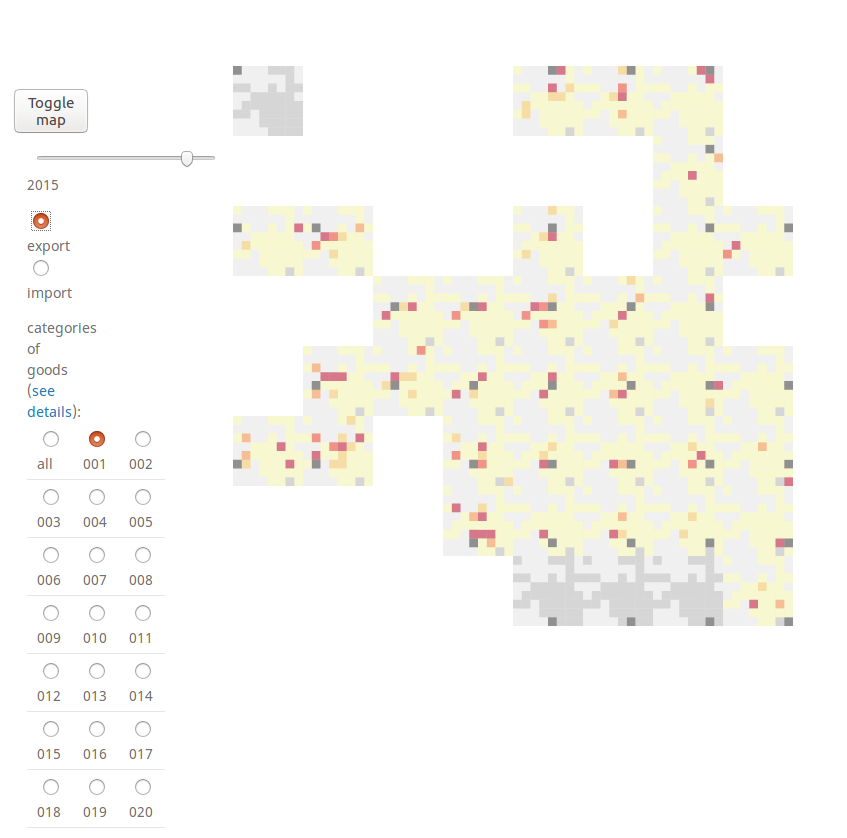
\includegraphics[scale=0.2]{OurMap.png}
\end{figure}

\section{Introduction}
In 2015, 323 billions of t-km of goods has been transported in Europe [1]. This freight is highly dominated by the road freight, representing more than 75 percent of the total freight. In this context, it could be interesting to produce visualization about this type of transport. It would be useful for different type of people, from beginners who just want to know a little more about road freight to professional that want to optimize their activities.
The goal is to highlight the biggest importers or exporters for each country, in general or by type of goods, and then the countries between which there is the more exchange. Then, several types of user could use this visualization for different purpose. 
Amateur users could only want to know from where comes the good they can consume, for example they could be interested in the majority provenance of the cigarettes they smoke, or the petroleum they use for their car.  
A more professional use of this visualization could be for a road transport company, which could then know which country to target if she wants to transport a certain type of good from a certain country.
Another use of this visualization would be in the economic or politic field, because the visualization spreads on eight years (from 2008 to 2016), so it could allow to see trends in import/export depending of the type of goods, the impact of a political change for a country, the impact of a climate disaster, or other event which can have an impact on the import/export dynamic for a country. 
Our visualization is able to combine a big quantity of information in only one map easily understandable by the user. Contrary to the visualization you can see on eurostat website [2], using OD maps allows the user to have a global view of the freight in Europe. Our system is much more specific (concentrated on one type of good for example) and, at the same time, more global with the total view of all country import or export in one chart. With our visualization, the user will have a high level of details and also a global view, because he will be able to see, with the same map and only by clicking on two buttons, the importation of oil in Sweden, and the exportation of manufactured goods in Austria. We could not find any maps or graphics on eurostat that gives at the same time this global view and these kind of details. In fact, bar chart visualization have already been made by Eurostat, to show for example the repartition of type of transport for each country for a particular year. However we did not found any map visualization that could summarize the data. Plus we did not found in this work any visualization concerning the exchanges between countries.


\section{Related Work}
An intuitive visualisation is proposed on the shipmap.org website \cite{shipmap} which focuses on maritime transports around the world. Each ship is represented by a dot of different colour according to the type of ship (Container, Tanker, Vehicle…). It looks like (at a larger scale) what we want to produce, but with some inconvenients. First, the type of goods is not detailed, because of the use of colours, which restrains the different representable types to a small number if we want to keep simplicity. Finally, there is no indication about the quantity of goods transported by each ship, so we don’t have information on the proportions of goods sent or received by each country. In this case, we don’t have the information on the quantity of goods that the ship carrying.

\begin{figure}[H]
\center
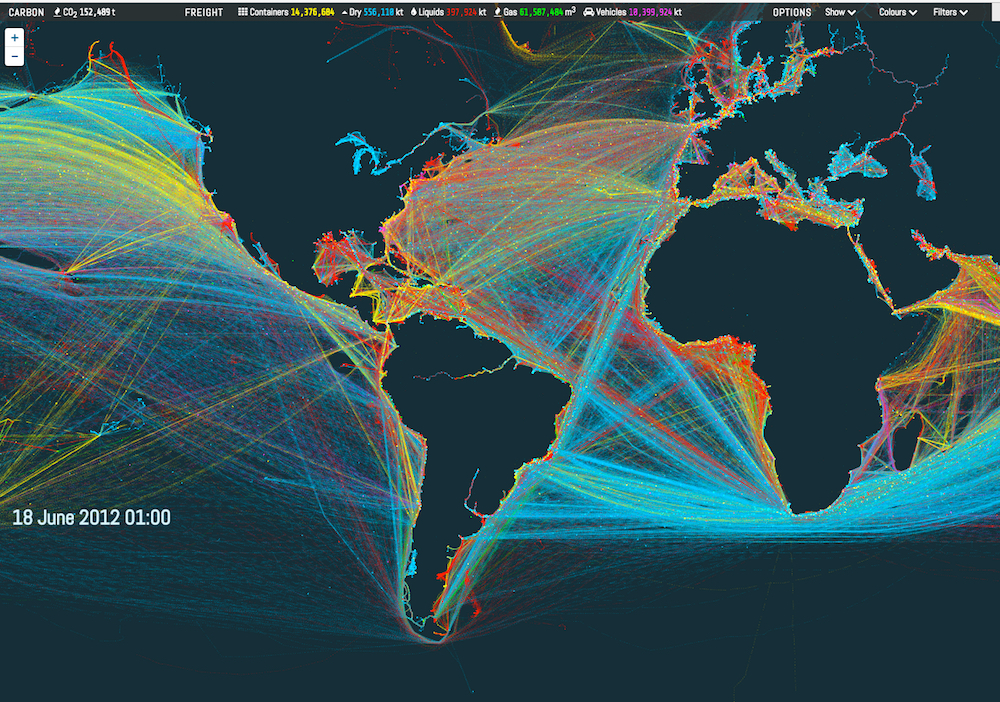
\includegraphics[scale=0.2]{shipmap.jpg}
\end{figure}

Furthermore, we’d like to keep the idea of a map as a function of time, to show the evolution of freight in UE for several years (depending on what is shown/the data used). 

Concerning network visualization, which we want to produce to show exchange between countries, we will base our work on visualizations produced by Martin Grandjean \cite{airtraffic}. This visualization is really good to show the principal localisation for the freight but it is way too complex to allow us to show the type of goods, or to differentiate importation and exportation. So we’ll have to simplify it before adding what we want to show in our visualization.

\begin{figure}[H]
\center
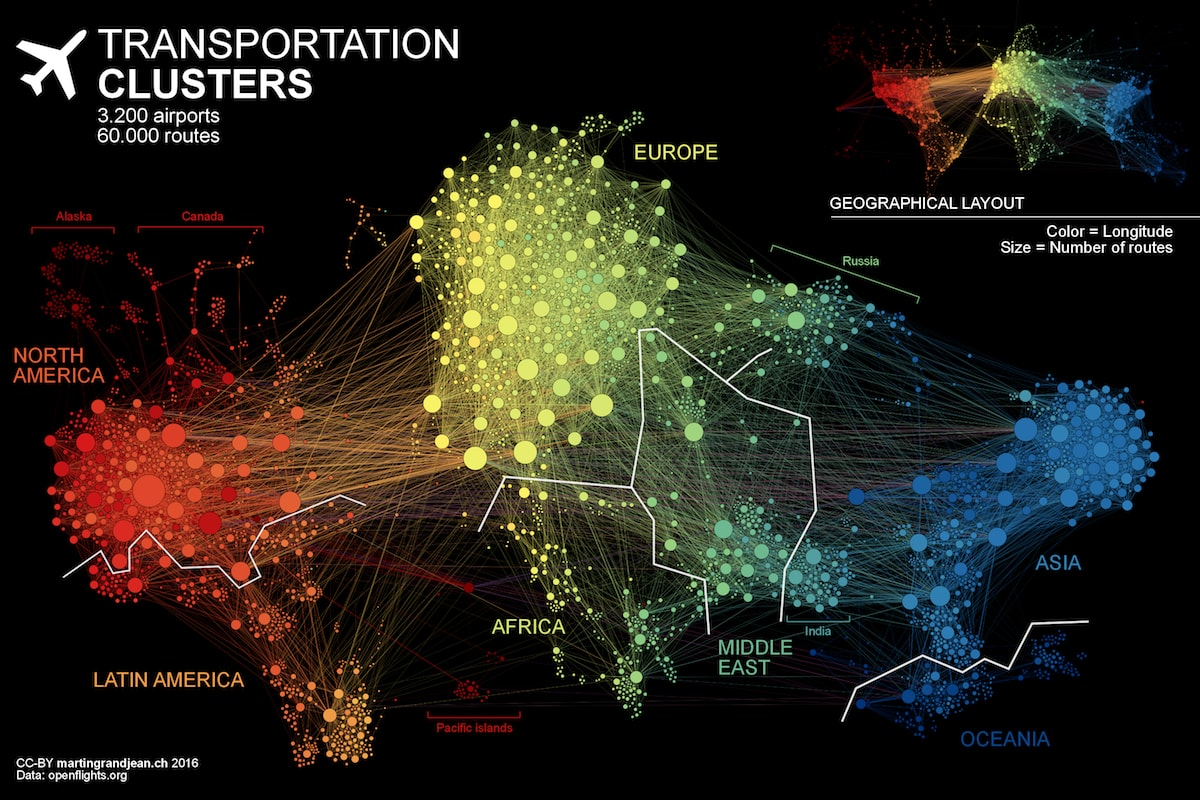
\includegraphics[scale=0.15]{airports-network-small.jpg}
\end{figure}

This third example of vizualisation shows another network. It’s presented in the atlas of economic complexity \cite{atlas}. Each node represents a product. It enables to present multiples products at once, but there is a single visualization for each country so it can be difficult if we want to compare countries between each other.

\begin{figure}[H]
\center
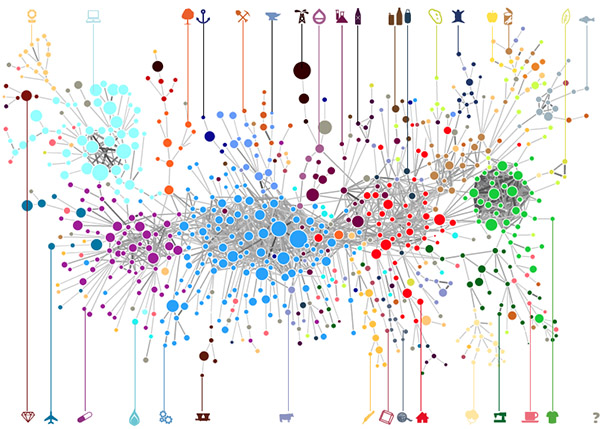
\includegraphics[scale=0.4]{economic_growth_atlas2.jpg}
\end{figure}


We choose to make an Origin-Destination map (OD map), because regarding the complixity and the amount of data we had, it seemed to be the simpliest way to show them without making a visualization not understandable easily. The principle of OD maps will be discussed later in the description of the project, but you can see an example here. 
\begin{figure}[H]
\center
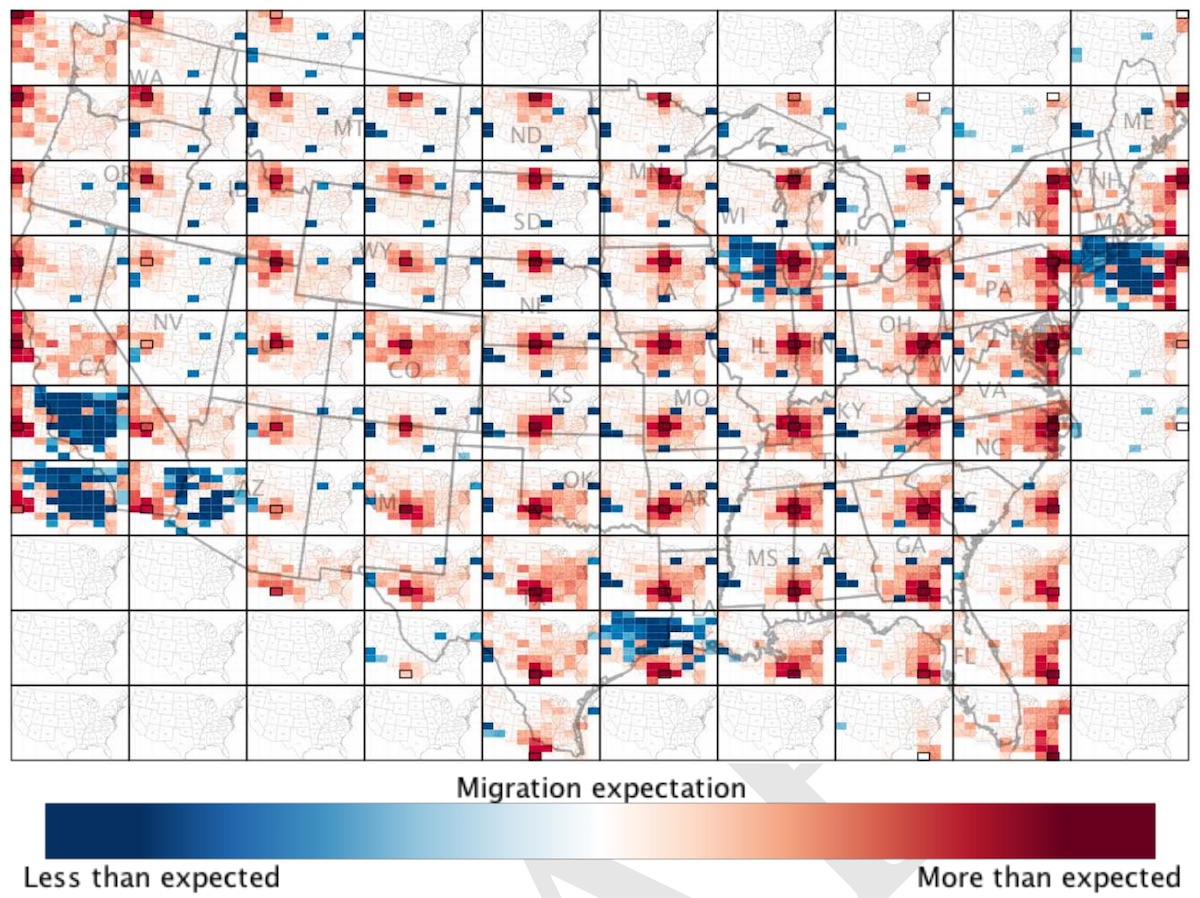
\includegraphics[scale=0.4]{odMap.jpg}
\end{figure}

% La ref de l'od map : http://www.maartenlambrechts.com/2017/05/03/the-eurosearch-song-contest-making-of.html


We decided to limit ourselves to the UE area and to focus on road freight, to keep the visualization simple by not adding too much information on it. Our work will be based on the one already done by the Eurostat organism, which has collected data about road, rail, sea and air freight in the European union. We will first focus on road freight (which represents about 75\% of the european freight \cite{dataset}).

\section{Project Description}

\subsection{Data}
We used the data provided by eurostat [2], on the annual road freight between european countries. At first they were in tsv format, so we had to parse them to make them usable in our visualization (get them in json format), and remove the unused data (for example, the data on exchange between country and the whole world). The parsing and production of json file have been done with python3 script. 

\subsection{Grid map}
A tile grid map or simple grid map is a representation of a geographic area divided into a set of equal squares\cite{Good Data Visualization Practice: Tile Grid Maps}.
The grid map is an unconventional choice to represent a geographic area but presents interesting advantages in our context. One of them is that it suppress the information of the size of the country, which is not relevant in our case, and can be a visual distorsion that leads the user to give more importance to largest countries. Furthermore, by simply represent each country by a square allows us to develop small multiple visualization (OD maps). You can notice that we add a toggle button that allow the user to change with an animation the grid map to the classic map with mercator projection. This allows the user to easily understand what is represented by the grid map and which square corresponds to each country. To make it even more simple, a tooltip appears when the users passes his mouse on a square, to indicate the name of the country. 


%on pourrait mettre 2 images : une de notre carte sous forme chloroplete et une de notre carte sous forme gridmap (mais sans les OD maps)
%keywords : #distortion #chloropleth 

\subsection{OD maps}
To Visualize the data, we choose to make OD maps. This consists of putting a little grid map in each square of the basic gridmap. From there, we can represent the exchange between countries. In each big square is represented a country, and in each little square in this big square is represented the other countries of our map. The coulour represents the quantity of goods imported (or exported, depending on what is chosen by the user) by the big square country from (or to, for exportation) the little square country. 
This type of visualisation brings a lot of advantages. First, it allows us to represent each countries by simple shape instead of a map where every country is different from the others. It is then easiest to apprehend for the user than if we had numerous different shapes. Second, integration of maps of europe in each square enable the identification of a pattern by the users, and then facilitates the comparison between two countries. It is notable to observe that it is feasible to make it because we only have about thirty countries. It would be a totally inapprehensible visualization if we applied these principles to a map of the entire world. The principle inconvenient with this visualization is that it is not obvious for the user that he is looking at the Europe, that is why we added the european map and the animation to let him know first what he is looking before truly looking at it. The tooltip on each country is also added in that way, to facilitate his navigation and not have to switch between geographical map and grid map. 

\subsection{Colors}
As explained before, we have an OD map, which means grid map inside our grid map, so the user can easily find the link between two countries. The quantity of good transported is represented by the intensity of the color in the little square. Here, we made the choice to put color intensity regarding to the maximum exchange of the country, and not the global maximum. For example, Netherland can have an importation of fifteen tkm from France for a type of good, and Germany have a hundred tkm for the same type, and each corresponding square can have the same color if fifteen is the maximum for this type for Netherland and a hundred is the maximum for Germany. We made this choice to avoid the colors to be overwritten by the countries like France, Germany of the United Kingdom which are bigger and economically more active than countries like Albania or Estonia. 

\subsection{Features}
To make it easy for the user to navigate between the data, and allow him to switch between the numerous type of goods and the two type of freight (import and export), we added two checkbox, one for the type of goods and one for the type of freight. In the one for the type of good, we added an “all” checkbox, to make it possible to view the total data. Plus, to navigate between the year, we added an horizontal scrollbar, to represent the timeline. We made these features this way because it seemed to be the easiest to understand and use for the user. 




\section{Discussion}
In regard to the complexity and the quantity of data, make a visualization easy tu use, understandable and efficient was challenging. Develop a visualization capable of contain all the exchanges between all countries for a year, and keep it readable on a single map demanded reflection and organisation. The visualization we produced allows to easily highlight trends if there is, to analyze quickly the evolution in time of the freight for one or several countries at the same time, and to switch quickly and easily between type of goods and of freight. For example, we can see, that the total quantity of exchange among two countries is pretty steady over time. By contrast, on a local scale (for a type of good in particular), we can see differences with lot more variation among the years and the type of good. This organisation let the user free to go depending of his own requirements.
One critic that can be made on this visualization is the choice explained before concerning the colors. In fact, it avoids the user to make a direct comparison between countries regarding the raw quantity (with direct tkm numbers). 
To get a more detailed dataset could also be interesting, because here we can say that we see a difference in the agriculture products, but we can not say from which product in particular of if it is a global pattern.


\section{Conclusion \& Perspectives}
We did not found any map visualization for the road freight, or at least not on the eurostat website, it was then interesting to make one. The quantity and the complexity of the data made really challenging to keep simplicity in the visualization and to allows the user to understand easily what he sees. We made it by combining animation (from geographical map to OD maps, to make it obvious that it is the Europe he is looking at), tooltip, and a simple way to show data, which was the OD map. Plus, if he looks for more details, he can find them on the same map, because it contains every exchanges found in the data between each countries on our map. So it can lead to a lot of different analyzes. 


\bibliographystyle{plain}
\bibliography{template}
\end{document}



Reference 
[1] ROAD FREIGHT TRANSPORT IS VITAL FOR EuropeAN ECONOMY European transport is : 24 billion tons of freight/year which 18 75 % of goods in term of volume billion tons/year transportED BY TRUCKS Transported by : 404 187 companies 251 506 m million euros (EU-15) ( (EU-15) -2,4% +13,8% between 2005 and 2010 (EU-15) between 2005 and 2010 (EU-15) WITH Drived by 7,8 Million Trucks About 4 > 3,5t * Millions Drivers * The number of employed drivers is estimated to be between 3.5 and 4 million based on French figures, number of vehicles and tonnage. With a traffic OF : World : 10 1 734 000 billion of tkm China : billion of tkm in 2011 5 137 1,3% annual growth between 1995 and 2003 billion of tkm USA : 1 929 billion of tkm Top ranking country In T-km/year +15% since 2000 323,83 DE +65% since 2000 PL 207,65 +29% since 2000 ES 206,84 -8% since 2000 FR 185,69 -8% since 2000 UK 152,99 Sources: European Commission, EU transport in figures, statistical pocketbook 2013; European Commission, EU energy and transport in figures 2007 www.michelin-solutions.com
[2] http://ec.europa.eu/eurostat/fr/home
